\hypertarget{ux5b57ux7b26ux4e32ux548cux7f16ux7801}{%
\subsection{字符串和编码}\label{ux5b57ux7b26ux4e32ux548cux7f16ux7801}}

\hypertarget{ux5b57ux7b26ux7f16ux7801}{%
\subsubsection{字符编码}\label{ux5b57ux7b26ux7f16ux7801}}

我们已经讲过了,字符串也是一种数据类型,但是,字符串比较特殊的是还有一个编码问题。

因为计算机只能处理数字,如果要处理文本,就必须先把文本转换为数字才能处理。最早的计算机在设计时采用
8
个比特(bit)作为一个字节(byte),所以,一个字节能表示的最大的整数就是
255(二进制 11111111 = 十进制
255),如果要表示更大的整数,就必须用更多的字节。比如两个字节可以表示的最大整数是\texttt{65535},4
个字节可以表示的最大整数是\texttt{4294967295}。

由于计算机是美国人发明的,因此,最早只有 127
个字符被编码到计算机里,也就是大小写英文字母、数字和一些符号,这个编码表被称为\texttt{ASCII}编码,比如大写字母\texttt{A}的编码是\texttt{65},小写字母\texttt{z}的编码是\texttt{122}。

但是要处理中文显然一个字节是不够的,至少需要两个字节,而且还不能和 ASCII
编码冲突,所以,中国制定了\texttt{GB2312}编码,用来把中文编进去。

你可以想得到的是,全世界有上百种语言,日本把日文编到\texttt{Shift\_JIS}里,韩国把韩文编到\texttt{Euc-kr}里,各国有各国的标准,就会不可避免地出现冲突,结果就是,在多语言混合的文本中,显示出来会有乱码。

 
 \begin{figure}[htp]
	\centering
	
\includegraphics[width=0.6\linewidth]{fig/9239304719270080.png}
\end{figure}


因此,Unicode 字符集应运而生。Unicode
把所有语言都统一到一套编码里,这样就不会再有乱码问题了。

Unicode 标准也在不断发展,但最常用的是 UCS-16
编码,用两个字节表示一个字符(如果要用到非常偏僻的字符,就需要 4
个字节)。现代操作系统和大多数编程语言都直接支持 Unicode。

现在,捋一捋 ASCII 编码和 Unicode 编码的区别:ASCII 编码是 1 个字节,而
Unicode 编码通常是 2 个字节。

字母\texttt{A}用 ASCII
编码是十进制的\texttt{65},二进制的\texttt{01000001};

字符\texttt{0}用 ASCII
编码是十进制的\texttt{48},二进制的\texttt{00110000},注意字符\texttt{\textquotesingle{}0\textquotesingle{}}和整数\texttt{0}是不同的;

汉字\texttt{中}已经超出了 ASCII 编码的范围,用 Unicode
编码是十进制的\texttt{20013},二进制的\texttt{01001110\ 00101101}。

你可以猜测,如果把 ASCII 编码的\texttt{A}用 Unicode 编码,只需要在前面补
0 就可以,因此,\texttt{A}的 Unicode 编码是\texttt{00000000\ 01000001}。

新的问题又出现了:如果统一成 Unicode
编码,乱码问题从此消失了。但是,如果你写的文本基本上全部是英文的话,用
Unicode 编码比 ASCII
编码需要多一倍的存储空间,在存储和传输上就十分不划算。

所以,本着节约的精神,又出现了把 Unicode 编码转化为 ``可变长编码''
的\texttt{UTF-8}编码。UTF-8 编码把一个 Unicode
字符根据不同的数字大小编码成 1-6 个字节,常用的英文字母被编码成 1
个字节,汉字通常是 3 个字节,只有很生僻的字符才会被编码成 4-6
个字节。如果你要传输的文本包含大量英文字符,用 UTF-8 编码就能节省空间:

\begin{longtable}[]{@{}llll@{}}
\toprule
字符 & ASCII & Unicode & UTF-8 \\ \addlinespace
\midrule
\endhead
A & 01000001 & 00000000 01000001 & 01000001 \\ \addlinespace
中 & x & 01001110 00101101 & 11100100 10111000 10101101 \\ \addlinespace
\bottomrule
\end{longtable}

从上面的表格还可以发现,UTF-8 编码有一个额外的好处,就是 ASCII
编码实际上可以被看成是 UTF-8 编码的一部分,所以,大量只支持 ASCII
编码的历史遗留软件可以在 UTF-8 编码下继续工作。

搞清楚了 ASCII、Unicode 和 UTF-8
的关系,我们就可以总结一下现在计算机系统通用的字符编码工作方式:

在计算机内存中,统一使用 Unicode
编码,当需要保存到硬盘或者需要传输的时候,就转换为 UTF-8 编码。

用记事本编辑的时候,从文件读取的 UTF-8 字符被转换为 Unicode
字符到内存里,编辑完成后,保存的时候再把 Unicode 转换为 UTF-8
保存到文件:

 
 \begin{figure}[htp]
	\centering
	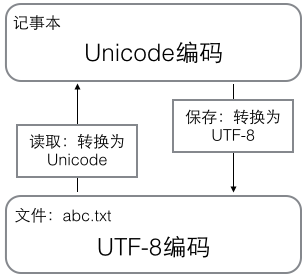
\includegraphics[width=0.6\linewidth]{fig/9239237870188160.png}
\end{figure}


浏览网页的时候,服务器会把动态生成的 Unicode 内容转换为 UTF-8
再传输到浏览器:

 
 \begin{figure}[htp]
	\centering
	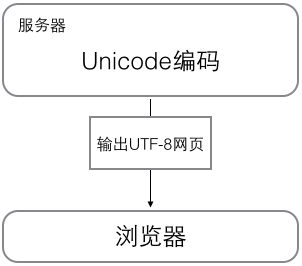
\includegraphics[width=0.6\linewidth]{fig/9239237591896000.png}
\end{figure}


所以你看到很多网页的源码上会有类似\texttt{\textless{}meta\ charset="UTF-8"\ /\textgreater{}}的信息,表示该网页正是用的
UTF-8 编码。

\hypertarget{python-ux7684ux5b57ux7b26ux4e32}{%
\subsubsection{Python 的字符串}\label{python-ux7684ux5b57ux7b26ux4e32}}

搞清楚了令人头疼的字符编码问题后,我们再来研究 Python 的字符串。

在最新的 Python 3 版本中,字符串是以 Unicode 编码的,也就是说,Python
的字符串支持多语言,例如:

\begin{pythoncode}
>>> print('包含中文的str')
包含中文的str
\end{pythoncode}

对于单个字符的编码,Python
提供了\texttt{ord()}函数获取字符的整数表示,\texttt{chr()}函数把编码转换为对应的字符:

\begin{pythoncode}
>>> ord('A')
65
>>> ord('中')
20013
>>> chr(66)
'B'
>>> chr(25991)
'文'
\end{pythoncode}

如果知道字符的整数编码,还可以用十六进制这么写\texttt{str}:

\begin{pythoncode}
>>> '\u4e2d\u6587'
'中文'
\end{pythoncode}

两种写法完全是等价的。

由于 Python 的字符串类型是\texttt{str},在内存中以 Unicode
表示,一个字符对应若干个字节。如果要在网络上传输,或者保存到磁盘上,就需要把\texttt{str}变为以字节为单位的\texttt{bytes}。

Python
对\texttt{bytes}类型的数据用带\texttt{b}前缀的单引号或双引号表示:

\begin{pythoncode}
x = b'ABC'
\end{pythoncode}

要注意区分\texttt{\textquotesingle{}ABC\textquotesingle{}}和\texttt{b\textquotesingle{}ABC\textquotesingle{}},前者是\texttt{str},后者虽然内容显示得和前者一样,但\texttt{bytes}的每个字符都只占用一个字节。

以 Unicode
表示的\texttt{str}通过\texttt{encode()}方法可以编码为指定的\texttt{bytes},例如:

\begin{pythoncode}
>>> 'ABC'.encode('ascii')
b'ABC'
>>> '中文'.encode('utf-8')
b'\xe4\xb8\xad\xe6\x96\x87'
>>> '中文'.encode('ascii')
Traceback (most recent call last):
  File "<stdin>", line 1, in <module>
UnicodeEncodeError: 'ascii' codec can't encode characters in position 0-1: ordinal not in range(128)
\end{pythoncode}

纯英文的\texttt{str}可以用\texttt{ASCII}编码为\texttt{bytes},内容是一样的,含有中文的\texttt{str}可以用\texttt{UTF-8}编码为\texttt{bytes}。含有中文的\texttt{str}无法用\texttt{ASCII}编码,因为中文编码的范围超过了\texttt{ASCII}编码的范围,Python
会报错。

在\texttt{bytes}中,无法显示为 ASCII
字符的字节,用\texttt{\textbackslash{}x\#\#}显示。

反过来,如果我们从网络或磁盘上读取了字节流,那么读到的数据就是\texttt{bytes}。要把\texttt{bytes}变为\texttt{str},就需要用\texttt{decode()}方法:

\begin{pythoncode}
>>> b'ABC'.decode('ascii')
'ABC'
>>> b'\xe4\xb8\xad\xe6\x96\x87'.decode('utf-8')
'中文'
\end{pythoncode}

如果\texttt{bytes}中包含无法解码的字节,\texttt{decode()}方法会报错:

\begin{pythoncode}
>>> b'\xe4\xb8\xad\xff'.decode('utf-8')
Traceback (most recent call last):
  ...
UnicodeDecodeError: 'utf-8' codec can't decode byte 0xff in position 3: invalid start byte
\end{pythoncode}

如果\texttt{bytes}中只有一小部分无效的字节,可以传入\texttt{errors=\textquotesingle{}ignore\textquotesingle{}}忽略错误的字节:

\begin{pythoncode}
>>> b'\xe4\xb8\xad\xff'.decode('utf-8', errors='ignore')
'中'
\end{pythoncode}

要计算\texttt{str}包含多少个字符,可以用\texttt{len()}函数:

\begin{pythoncode}
>>> len('ABC')
3
>>> len('中文')
2
\end{pythoncode}

\texttt{len()}函数计算的是\texttt{str}的字符数,如果换成\texttt{bytes},\texttt{len()}函数就计算字节数:

\begin{pythoncode}
>>> len(b'ABC')
3
>>> len(b'\xe4\xb8\xad\xe6\x96\x87')
6
>>> len('中文'.encode('utf-8'))
6
\end{pythoncode}

可见,1 个中文字符经过 UTF-8 编码后通常会占用 3 个字节,而 1
个英文字符只占用 1 个字节。

在操作字符串时,我们经常遇到\texttt{str}和\texttt{bytes}的互相转换。为了避免乱码问题,应当始终坚持使用
UTF-8 编码对\texttt{str}和\texttt{bytes}进行转换。

由于 Python
源代码也是一个文本文件,所以,当你的源代码中包含中文的时候,在保存源代码时,就需要务必指定保存为
UTF-8 编码。当 Python 解释器读取源代码时,为了让它按 UTF-8
编码读取,我们通常在文件开头写上这两行:

第一行注释是为了告诉 Linux/OS X 系统,这是一个 Python
可执行程序,Windows 系统会忽略这个注释;

第二行注释是为了告诉 Python 解释器,按照 UTF-8
编码读取源代码,否则,你在源代码中写的中文输出可能会有乱码。

申明了 UTF-8 编码并不意味着你的\texttt{.py}文件就是 UTF-8
编码的,必须并且要确保文本编辑器正在使用 UTF-8 without BOM 编码:

 
 \begin{figure}[htp]
	\centering
	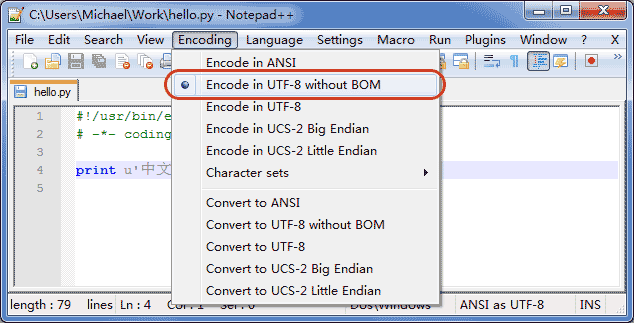
\includegraphics[width=0.6\linewidth]{fig/1008802356788736.png}
\end{figure}


如果\texttt{.py}文件本身使用 UTF-8
编码,并且也申明了\texttt{\#\ -*-\ coding:\ utf-8\ -*-},打开命令提示符测试就可以正常显示中文:

 
 \begin{figure}[htp]
	\centering
	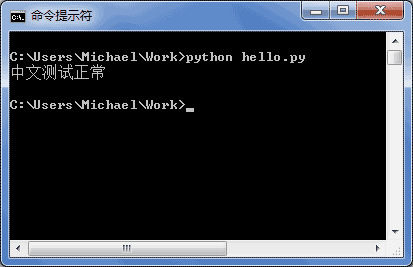
\includegraphics[width=0.6\linewidth]{fig/1008802515054144.png}
\end{figure}


\hypertarget{ux683cux5f0fux5316}{%
\subsubsection{格式化}\label{ux683cux5f0fux5316}}

最后一个常见的问题是如何输出格式化的字符串。我们经常会输出类似\texttt{\textquotesingle{}亲爱的xxx你好!你xx月的话费是xx,余额是xx\textquotesingle{}}之类的字符串,而
xxx 的内容都是根据变量变化的,所以,需要一种简便的格式化字符串的方式。

 
 \begin{figure}[htp]
	\centering
	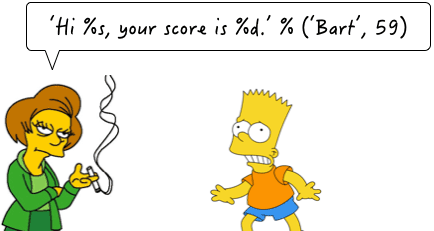
\includegraphics[width=0.6\linewidth]{fig/9288179064464320.png}
\end{figure}


在 Python 中,采用的格式化方式和 C
语言是一致的,用\texttt{\%}实现,举例如下:

\begin{pythoncode}
>>> 'Hello, %s' % 'world'
'Hello, world'
>>> 'Hi, %s, you have $%d.' % ('Michael', 1000000)
'Hi, Michael, you have $1000000.'
\end{pythoncode}

你可能猜到了,\texttt{\%}运算符就是用来格式化字符串的。在字符串内部,\texttt{\%s}表示用字符串替换,\texttt{\%d}表示用整数替换,有几个\texttt{\%?}占位符,后面就跟几个变量或者值,顺序要对应好。如果只有一个\texttt{\%?},括号可以省略。

常见的占位符有:

\begin{longtable}[]{@{}ll@{}}
\toprule
占位符 & 替换内容 \\ \addlinespace
\midrule
\endhead
\%d & 整数 \\ \addlinespace
\%f & 浮点数 \\ \addlinespace
\%s & 字符串 \\ \addlinespace
\%x & 十六进制整数 \\ \addlinespace
\bottomrule
\end{longtable}

其中,格式化整数和浮点数还可以指定是否补 0 和整数与小数的位数:

\begin{pythoncode}
# -*- coding: utf-8 -*-
\end{pythoncode}

如果你不太确定应该用什么,\texttt{\%s}永远起作用,它会把任何数据类型转换为字符串:

\begin{pythoncode}
>>> 'Age: %s. Gender: %s' % (25, True)
'Age: 25. Gender: True'
\end{pythoncode}

有些时候,字符串里面的\texttt{\%}是一个普通字符怎么办?这个时候就需要转义,用\texttt{\%\%}来表示一个\texttt{\%}:

\begin{pythoncode}
>>> 'growth rate: %d %%' % 7
'growth rate: 7 %'
\end{pythoncode}

\hypertarget{format}{%
\subsubsection{format()}\label{format}}

另一种格式化字符串的方法是使用字符串的\texttt{format()}方法,它会用传入的参数依次替换字符串内的占位符\texttt{\{0\}}、\texttt{\{1\}}\ldots\ldots,不过这种方式写起来比
\% 要麻烦得多:

\begin{pythoncode}
>>> 'Hello, {0}, 成绩提升了 {1:.1f}%'.format('小明', 17.125)
'Hello, 小明, 成绩提升了 17.1%'
\end{pythoncode}

\hypertarget{f-string}{%
\subsubsection{f-string}\label{f-string}}

最后一种格式化字符串的方法是使用以\texttt{f}开头的字符串,称之为\texttt{f-string},它和普通字符串不同之处在于,字符串如果包含\texttt{\{xxx\}},就会以对应的变量替换:

\begin{pythoncode}
>>> r = 2.5
>>> s = 3.14 * r ** 2
>>> print(f'The area of a circle with radius {r} is {s:.2f}')
The area of a circle with radius 2.5 is 19.62
\end{pythoncode}

上述代码中,\texttt{\{r\}}被变量\texttt{r}的值替换,\texttt{\{s:.2f\}}被变量\texttt{s}的值替换,并且\texttt{:}后面的\texttt{.2f}指定了格式化参数(即保留两位小数),因此,\texttt{\{s:.2f\}}的替换结果是\texttt{19.62}。

\hypertarget{ux7ec3ux4e60}{%
\subsubsection{练习}\label{ux7ec3ux4e60}}

小明的成绩从去年的 72 分提升到了今年的 85
分,请计算小明成绩提升的百分点,并用字符串格式化显示出\texttt{\textquotesingle{}xx.x\%\textquotesingle{}},只保留小数点后
1 位:

\begin{pythoncode}
# -*- coding: utf-8 -*-

s1 = 72
s2 = 85
\end{pythoncode}

\hypertarget{ux5c0fux7ed3}{%
\subsubsection{小结}\label{ux5c0fux7ed3}}

Python 3 的字符串使用 Unicode,直接支持多语言。

当\texttt{str}和\texttt{bytes}互相转换时,需要指定编码。最常用的编码是\texttt{UTF-8}。Python
当然也支持其他编码方式,比如把 Unicode 编码成\texttt{GB2312}:

\begin{pythoncode}
>>> '中文'.encode('gb2312')
b'\xd6\xd0\xce\xc4'
\end{pythoncode}

但这种方式纯属自找麻烦,如果没有特殊业务要求,请牢记仅使用\texttt{UTF-8}编码。

格式化字符串的时候,可以用 Python 的交互式环境测试,方便快捷。

\hypertarget{ux53c2ux8003ux6e90ux7801}{%
\subsubsection{参考源码}\label{ux53c2ux8003ux6e90ux7801}}

\href{https://github.com/michaelliao/learn-python3/blob/master/samples/basic/the_string.py}{the\_string.py}

